% Chapter Template

\chapter{Sensory Redundancy: Are Two Heads Better Than One?} % Main chapter title

\label{Chapter4} % Change X to a consecutive number; for referencing this chapter elsewhere, use \ref{ChapterX}

\lhead{Chapter 4. \emph{Sensory Redundancy: Are Two Heads Better Than One?}} % Change X to a consecutive number; this is for the header on each page - perhaps a shortened title

%----------------------------------------------------------------------------------------
%	SECTION 1
%----------------------------------------------------------------------------------------

\section{Why Have One Sensor When Two Are Better?}
A key part of the human experience is that it is multisensory. In \cite{barsalou2008grounded}, Lawrence Barsalou speaks about how multisensory processing aids human cognition in a number of ways. Firstly, multisensory information aids in the classification of experiences by providing additional and complimentary information that is not accounted for in only a single modality. 

Lip reading affects the classification of phonemes, this is known as the Mcgurk effect \cite{mcgurk1976hearing}. Whilst this effect can lead to incorrect classifications when misaligned data is provided e.g. utterances of the syllable [ba] dubbed on to lip movements for [ga], lead to normal adults hearing [da]; in normal circumstances, like when two people are speaking to one and other, lip reading aids in classifying heard sounds \cite{ma2009lip}. This is particularly important in noisy environments, which leads to another of Barsalou's ideas about multisensory processing: information redundancy.

The reason that lip reading can aid hearing in noisy evironments is that it provides an additional vector along which the human brain can reconstruct missing information. When something is mis-heard due to background noise, the visual information gained from looking at the lips of the speaker can be used to reconstruct their utterance.

The ability to reconstruct missing data from a secondary modality has not only been seen in humans \cite{ma2009lip, samuel1997lexical} but has been demonstrated in computational modals for example,\cite{ngiam2011multimodal, silberer2014learning}.

In order to be able to reconstruct missing data from a secondary modality, symbol grounding needs to have occured, and the meaning of a percept in modality A must be known in modality B.
If both the forward and inverse relationship between modalities is known, then bidirectional symbol grounding has occured and we are able to reconstruct modality A from modality B and modality B from modality A.

In this chapter I will explore these two ideas, improved classification and reconstruction of missing information through  bidirectional symbol grounding using \acp{MAE}.



\section{Generating Images From Natural Language}
\subsection{Aims}
The experiment in this section demonstrates that having access to a second modality improves classification accuracy over the baseline accuracy of classification of either of the two individual modalities as well as how missing data can be reconstructed from a secondary modality. \textcolor{red}{Whilst the methodology followed in this chapter matches that of \cite{ngiam2011multimodal} and \cite{silberer2014learning}, I make use of different data modalities, explore the quality of images generated by the \ac{MAE} and test different methods for combining the individual representations of the two modalities into a joint representation.}

\textcolor{The main aims of the experiments in this chapter are to find the best method for producing the joint representation of the two different data sources, and also proving hypothesis 1: \ac{MRL} can be used to learn the association between sounds and the visual symbols they represent and hypothesis 2: \ac{MRL} enhances classification accuracy of sounds and visual symbols.}

\subsection{A note on Qualatitive Anaylsis of Image Generation}
\textcolor{red}{As quantitive analysis is difficult, I will make use of a qualititive analysis to describe the quality of the images generated in this and subsequent chapters.
This is in line with the the analysis performed in \cite{reed2016generative, zhang2017stackgan, xu2018attngan, li2018video, mansimov2015generating} in which human analysis of generated images is used.}

\textcolor{red}{However \cite{zhang2017stackgan, xu2018attngan, li2018video} also make use of Inception score to provide a quantitive measure of the images they generate. Inception score is the \ac{KLD} between $P(y|x)$ and $P(y)$ where $x$ is a generated image and $y$ is a class label generated by a pretrained classifier (\cite{zhang2017stackgan, xu2018attngan, li2018video} make use of the Inception net \cite{szegedy2017inception} for this classification, hence the name of their metric.}

\textcolor{red}{Inception score is not suitable for my purposes for two main reasons. 1) I do not have pretrained classifiers for the datasets used in this thesis and 2) Inception score only indicates whether a generated image can be classified into a particular category, it does not indicated whether the image matches the description from which it was generated as noted by Zhang et al in \cite{zhang2017stackgan}.}

\begin{displayquote}
\textcolor{red}{Although the inception score has shown to well correlate
with human perception on visual quality of samples, it
cannot reflect whether the generated images are well con-
ditioned on the given text descriptions.}
- Zhang et al.
\end{displayquote}

\textcolor{red}{In order to make the qualititive analysis of generated images more precise, I will comment on image properties such as image noise, including sharpness/blurriness and salt-and-pepper noise. I will also comment on whether the generated images are recognisable as belonging to the category to which they should belong.} 

\subsection{UCU Arabic Spoken Digits and MNIST} 
\label{sec:UCU}
This experiment utilises two datasets, UCU Arabic Spoken Digits (UCU) and MNIST Handwritten Digits (MNIST).

\subsubsection{UCU Arabic Spoken Digits}
UCU is a dataset containing the 13 \acp{MFCC} representing the audio of the digits 0 to 9 being said by 88 different speakers \cite{hammami2009tree,hammami2010improved}. It contains 8800 utterances (10 digits x 10 repetitions x 88 speakers). Audio was sampled at 11025Hz.

\paragraph{Padding of Utterances}
As utterances are not of a fixed length, it is necessary to pad the utterances to be equal length. The longest utterance in the dataset contains 93 samples. For ease of up and downsampling within the neural network, all uttereances are padded to be 100 samples long by appending zeros. Each sample is also padded to contain 16 features, the 13 \acp{MFCC} and 3 zeros to further facilitate up and down sampling. Up and down sampling is easier with even numbers of features and samples as we can half the size of the data using strided convolutions, s=(2,2), without worrying about integer division errors e.g. $5/2=2$ but $2\times2 \neq5$.

As I will be classifying the digits, it is necessary to check that padding the digits does not provide a cheat for this. As such, I analyse the mean number of samples for each digit and their standard deviations as depicted in \autoref{fig:ucu_dig_length}. I then perform a linear regression on the number of samples to demonstrate that it is not possible to accurately predict a digit's class given only the length of the utterance.

\begin{figure}
\centering
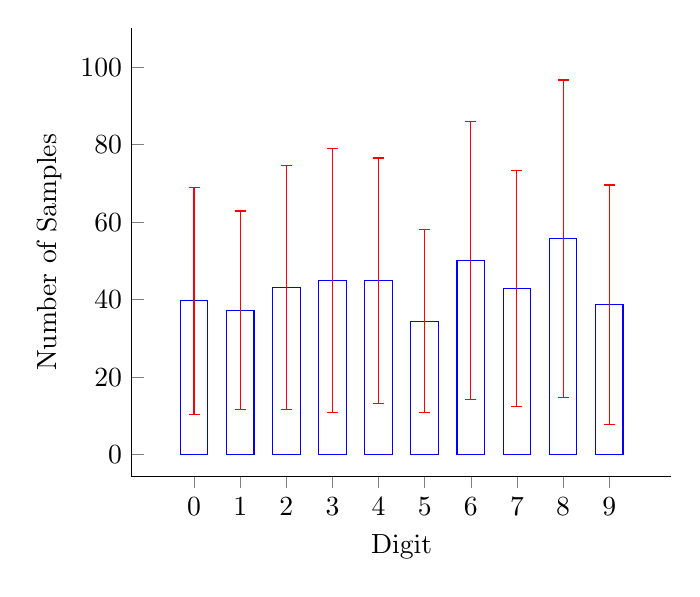
\begin{tikzpicture}
\begin{axis}[
	axis x line*=bottom,
	axis y line*=left,
	%at={(-1,0)}
    ybar,
    enlargelimits=0.15,
    ylabel={Number  of Samples},
    ytick={0,20,40,60,80, 100},   
    xtick={1,2,3,4,5,6,7,8,9,10},
    xticklabels={0,1,2,3,4,5,6,7,8,9}, %{zero, one, two, three, four, five, six, seven, eight, nine}
    %x tick label style={rotate=45},
    xlabel={Digit},
    %nodes near coords,
    %nodes near coords align={vertical},
    xlabel near ticks,
	ylabel near ticks,
	bar shift=0pt
    ]
%\addplot coordinates {(1,39.66) (2,37.27) (3,43.11) (4,45.02) (5,44.92) (6,34.44) (7,50.10) (8,42.81) (9,55.67) (10,38.63)};
\addplot[blue, error bars, y dir=both,y explicit, error bar style={color=red}]
 coordinates { 
(1,39.66) +- (0.0,29.25) 
(2,37.27) +- (0.0,25.58) 
(3,43.11) +- (0.0,31.43) 
(4,45.02) +- (0.0,34.05) 
(5,44.92) +- (0.0,31.63) 
(6,34.44) +- (0.0,23.63)
(7,50.10) +- (0.0,35.90)
(8,42.81) +- (0.0,30.41)
(9,55.67) +- (0.0,41.01)
(10,38.63) +- (0.0,30.94)
  };
\end{axis}
\end{tikzpicture}

	%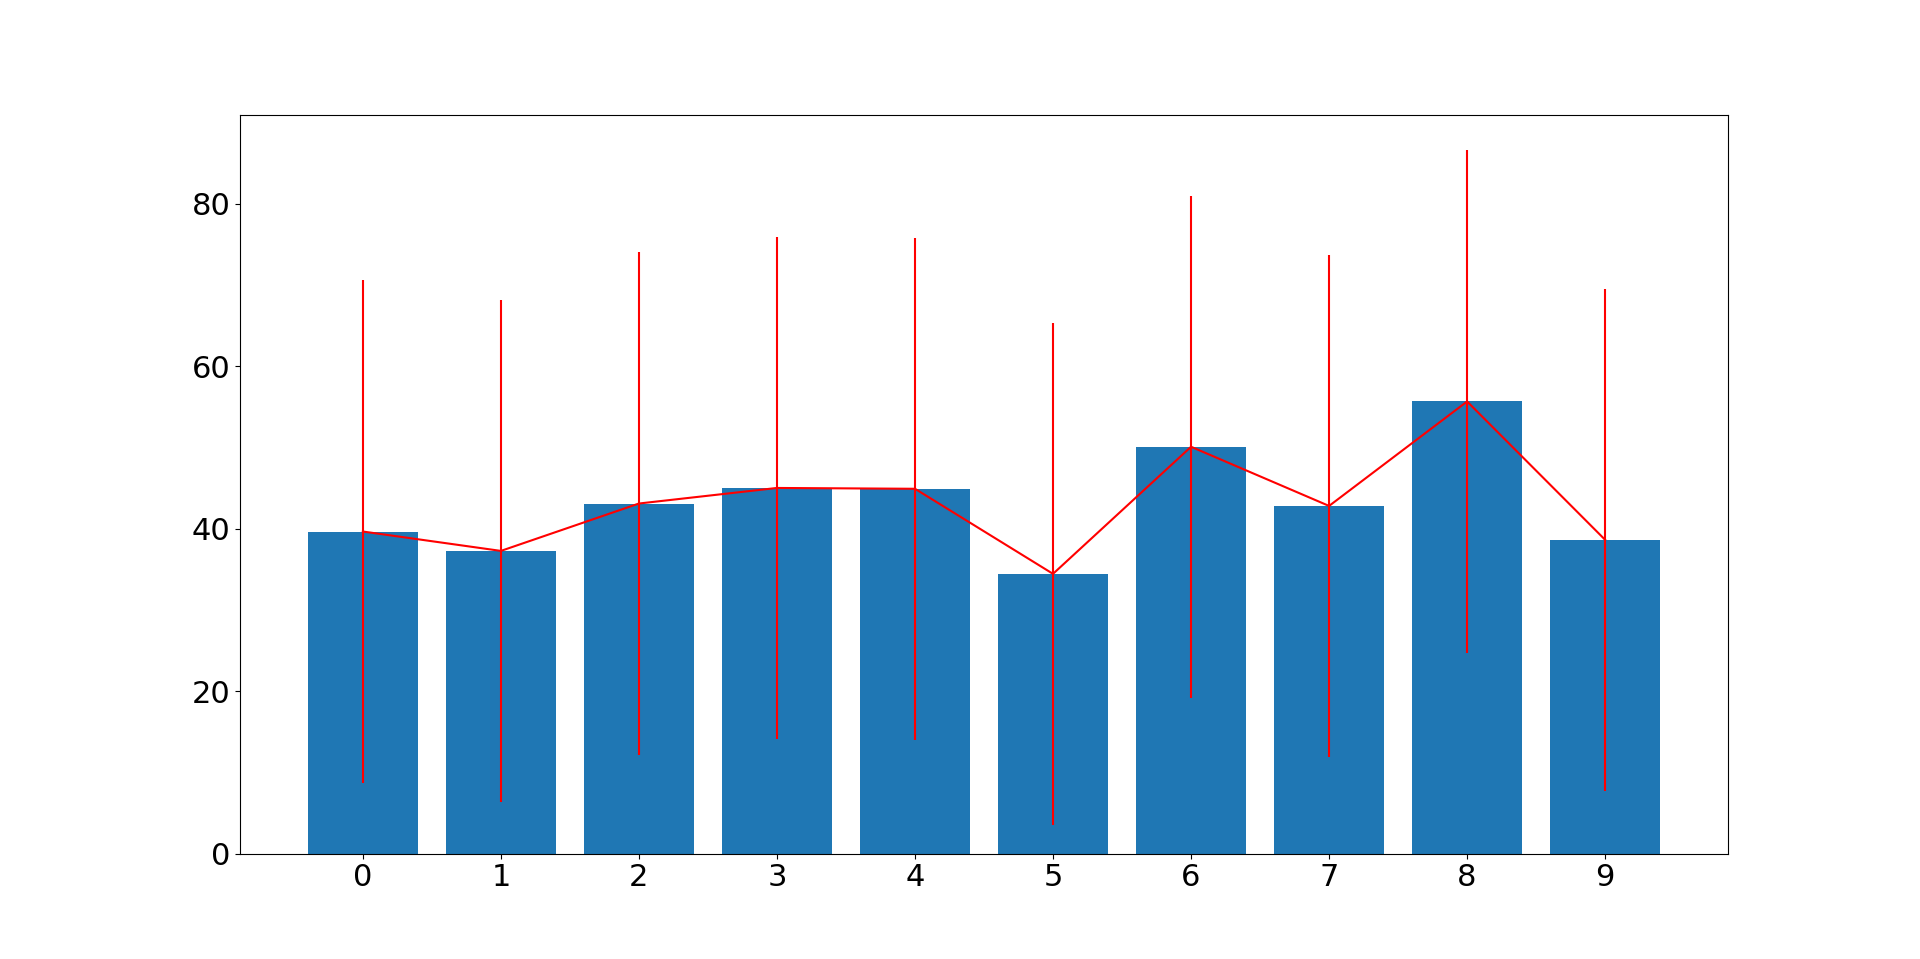
\includegraphics[width=\textwidth]{./Figs/mnistSpoken/UCU_digit_length.png}
	\caption{Mean number of samples for each digit in the UCU Arabic Spoken Digits Dataset. Red bars show the standard devaition in length for each each digit.}
	\label{fig:ucu_dig_length}

\end{figure}

\autoref{fig:ucu_dig_length} shows the mean number of samples for each digit in the UCU dataset. Whilst there is a difference in the mean length of each digit, the standard deviation for each digit is relatively large as can be seen in \autoref{tab:UCU_sampLen}. Therefore, trying to classifiy the digits just by the number of samples in an example, is ineffective.

	\begin{table}
		\centering
		\begin{tabular}{|c|c|c|}
			\hline
			\textbf{Digit} & \textbf{Mean Length (samples)} & \textbf{Standard Deviation} \\ \hline
			0 & 39.66 & $\mypm 29.25$ \\ \hline
			1 & 37.27 & $\mypm 25.58$ \\ \hline
			2 & 43.11 & $\mypm 31.43$ \\ \hline
			3 & 45.02 & $\mypm 34.05$ \\ \hline
			4 & 44.92 & $\mypm 31.63$ \\ \hline
			5 & 34.44 & $\mypm 23.63$ \\ \hline
			6 & 50.10 & $\mypm 35.90$ \\ \hline
			7 & 42.81 & $\mypm 30.41$ \\ \hline
			8 & 55.67 & $\mypm 41.01$ \\ \hline
			9 & 38.63 & $\mypm 30.94$ \\ \hline

		\end{tabular}
		\caption{Mean length and standard deviation of digits in the UCU dataset.}
		\label{tab:UCU_sampLen}
	\end{table}


Performing a linear regression on the number of samples for each digit versus its class, we get an accuracy of 6.18\% when classifying the test set.

\subsubsection{MNIST Handwritten Digits}
MNIST is a well known and oft used dataset in the machine learning community. It contains 60,000 training samples and 10,000 test samples, evenly split between the digits 0 to 9. 
Each digit is presented as a grey-scale, 28x28 pixel image \cite{lecun1998mnist}. 

\subsection{Problem Description}
The experiments with these datasets will explore two problems: classification and bidirectional symbol grounding. 

\subsubsection{Classification}
Each of the utterances and images from the UCU and MNIST datasets are classified as being a numeric digit, 0 to 9. By combining both datasets, I can explore whether the addition of a second modality enhances overall classification accuracy.

I start off exploring the classification abilities of neural networks by performing a linear regression with a single, dense neural network layer with a softmax activation on the activation of the embedding layer of an autoencoder, this is the neural networks representation of the digit. To generate baseline classification accuracies for each dataset, I use autoencoders for each modality separately.

Once a classification baseline has been established for each dataset, I make use of a \ac{MAE}, using paired examples from each dataset to train it.

\subsubsection{Bidirectional Symbol Grounding}

I demonstrate that a neural network can perform bidirectional symbol grounding \cite{barsalou2008grounded} when presented with aligned images and utterances. To explore this, I show how a \ac{MAE} can learn to reconstruct the correct image of a digit given the \acp{MFCC} of an utterance as well as \acp{MFCC} which have a small mean squared error from the correct utterance given an image of a digit. This shows that an internal symbolic language has been learnt in the form of the latent embedding created by the encoders of the \ac{MAE}.


\subsection{Experiment Details}
Images from the MNIST dataset are kept at their original scale of 28x28 pixels and are normalised such that each pixel has a value from 0 to 1 based on its intensity, with zero equating to black and 1 being white.

The UCU dataset is normalised so that all \acp{MFCC} take a value from 0 to 1 based on the value of the \ac{MFCC} such that the highest value is 1 and the lowest 0. Utterances are padded to be 100x16 as previously described.

\paragraph{Combining Datasets}
\label{sec:UCU_mnist_comb}
Due to the difference in size between the datasets, 8,800 samples for UCU and 70,000 samples for MNIST, I randomly sample from the UCU dataset and pair this with a sample from MNIST. This means that each sample from UCU is used approxiamtely 7.95 times ($70000/8800=7.9545$) in the training data.

\paragraph{Merging Modalities}
In order to combine the two different modalities, I explore different merging techniques: concatenation (\textit{Concat}) and addition (\textit{Add}). To do this, the embeddings of both modalities are ensured to have the same shape and then are merged using the methods described in \autoref{eqn:concat} and \autoref{eqn:add} for concatenation and addition, respectively. %and \ref{eqn:xply}.

 \begin{equation}\label{eqn:concat}
 	merged = Im_i^{emb} || MFCC_i^{emb} 	
 \end{equation}

 \begin{equation}\label{eqn:add}  
 	merged = Im_i^{emb} + MFCC_i^{emb} 	
 \end{equation}
 
  %\begin{equation}
 	%merged = x1^*_i * x2^*_i
 	%\label{eqn:xply}  
 %\end{equation}

Where $Im_i^{emb}$ and $MFCC_i^{emb}$ represent the embeddings, output by the image and \ac{MFCC} encoders respectively for image and \ac{MFCC} inputs $Im_i$ and $MFCC_i$.

\subsubsection{Training Procedures}

The \acp{MAE} are trained in two different ways for both types of merging, these are referred to as bimodal (Bi) and randomly removed (RR).

\paragraph{Bimodal}
Under the Bi training procedure, the \ac{MAE} is presented with bimodal input for all training instances. Both image and \ac{MFCC} inputs are present for all training steps and the \ac{MAE} is trained to reproduce this input as its output.

\paragraph{Randomly Removed}
Under the RR training procedure, one third of image inputs are removed at random and one third of \ac{MFCC} inputs are removed at random. It is ensured that each training instance always has at least one input modality present. That is, a training instance never has both its image and \ac{MFCC} input removed. 

The removed modality is replaced with an array of zeros of the same shape as the original input (28x28 for the image and 100x16 for \acp{MFCC}).

The \ac{MAE} is then trained to reproduce both the image and \acp{MFCC} regardless of whether one of these has been ommited from the input.

\subsubsection{Testing Conditions}
Each \ac{MAE} (\textit{Concat} and \textit{Add}) was tested in three different ways, Bimodal, Image Only and \ac{MFCC} Only.

\paragraph{Bimodal}
In the Bimodal testing condition both image and \ac{MFCC} data are used as input for each testing instance and I am interested in observing the classification accuracy as well as the total regeneration error.

\paragraph{Image Only}
In the Image Only testing condition, only images are provided as input data. I am interested in the classification accuracy as well as the \ac{MFCC} reconstruction error. I am not interested in the image reconstruction error, as it is expected that, as the image is provided as input this will be low (which it is for all models and training procedures as seen in \autoref{tab:mnist_ucu_master_res}).  

\paragraph{\ac{MFCC} Only}
Similarly to the Image Only condition, the \ac{MFCC} Only condition provides only \acp{MFCC} as input and I am interested in the classification accuracy as well as the image reconstruction error. I am not interested in the \ac{MFCC} regeneration loss as \acp{MFCC} are given as input it will be low (which it is for all models and training procedures as seen in \autoref{tab:mnist_ucu_master_res}).  

\subsubsection{Network Description}
\paragraph{Baseline Models}
To generate the baseline classification accuracies for both the UCU and MNIST data, I make use of (unimodal) autoencoders. The descrition of the autoencoder for the MNIST dataset can be found in \autoref{tab:MNIST_AE_description} and the autoencoder for the UCU dataset in \autoref{tab:UCU_AE_description}.

\textcolor{red}{The design of the unimodal autoencoders was achieved by attempting to maximise the classification accuracy of the MNIST and UCU datasets whilst minimising their reconstruction error. The decoder portion of the autoencoders was formed by flipping the encoder are replacing convolution layers with transposed convolutions, such that the network is symetrical and the generated output is of the same dimension as the input.}

	\begin{table}[th!]
		\centering
		\begin{tabular}{|c|c|c|c|c|c|c|}
			\hline
			\textbf{Block} & \textbf{Layer} & \textbf{Type} & \textbf{Neurons} & \textbf{Kernel} & \textbf{Strides} & \textbf{Activation}  \\ \hline
			\multirow{4}{*}{Encoder} & 1	&	2D Conv & 32 & (3,3) & (1,1)  & Relu\\ \cline{2-7}
			& 2	&	2D Conv & 64 & (3,3) & (2,2) & Relu \\ \cline{2-7}
			& 3	&	2D Conv & 64 & (3,3) & (2,2) & Relu \\ \cline{2-7}
			& 4 	&	Dropout p=0.25 &	 & 	     &       & \\ \hline
			Embedding & 5	&	2D Conv & 32 & (3,3) & (1,1) & Relu \\ \hline
			Classifier & 6c	&	Dense          & 10 &       &       & Softmax      \\ \hline
			\multirow{5}{*}{Decoder}& 6 	&	Dropout p=0.25 &	 & 	     &       & \\ \cline{2-7}
			& 7	&	2D Trans Convn & 64 & (3,3) & (2,2) & TanH \\ \cline{2-7}
			& 8	&	2D Transp Conv & 64 & (3,3) & (2,2) & TanH \\ \cline{2-7}
			& 9	&	2D Trans Conv & 32 & (3,3) & (1,1) & TanH \\ \cline{2-7}
			& 10	&	2D Trans Conv & 1 & (3,3) & (1,1) & Sigmoid \\ \hline
		\end{tabular}
		\caption{Image autoencoder and classifier. Layer 6c performs classification, whilst the branch starting at layer 6 regenerates the image.}
		\label{tab:MNIST_AE_description}
	\end{table}

	\begin{table}[h!]
		\centering
		\begin{tabular}{|c|c|c|c|c|c|c|}
			\hline
			\textbf{Block} & \textbf{Layer} & \textbf{Type} & \textbf{Neurons} & \textbf{Kernel} & \textbf{Strides} & \textbf{Activation}  \\ \hline
			\multirow{5}{*}{Encoder} & 1	&	2D Conv & 32 & (3,3) & (1,1)  & Relu\\ \cline{2-7}
			& 2	&	2D Conv & 64 & (3,3) & (2,2)  & Relu\\ \cline{2-7}
			& 3 	&	Dropout p=0.25 &	 & 	     &        & \\ \cline{2-7}
			& 4	&	Dense          & 3136 & 	 &        & \\ \cline{2-7}
			& 5   &	Reshape (7,7,64) &    &     &        & \\ \hline
			Embedding & 6	&	2D Conv & 32 & (3,3) & (1,1)  & Relu  \\ \hline
			Classifier & 7c	&	Dense          & 10 &       &        & Softmax \\ \hline
			\multirow{7}{*}{Decoder} & 7 	&	Dropout p=0.25 &	 & 	     &        & \\ \cline{2-7}
			& 9	&	Dense			& 3200 &     &        & \\ \cline{2-7}
			& 10	&	Reshape (25,4,32) &    &    &        & \\ \cline{2-7}
			& 11	&	2D Trans Conv & 64 & (3,3) & (2,2)  & TanH \\ \cline{2-7}
			& 12	&	2D Trans Conv & 64 & (3,3) & (2,2)  & TanH \\ \cline{2-7}
			& 13	&	2D Trans Conv & 32 & (3,3) & (1,1)  & TanH \\ \cline{2-7}
			& 14	&	2D Trans Conv & 1 & (3,3) & (1,1) & Sigmoid \\ \hline
		\end{tabular}
		\caption{\ac{MFCC} autoencoder and classifier. Layer 7c performs classification, whilst the branch starting at layer 7 regenerates the \acp{MFCC}. The addition of reshape layers is to ensure the final shape of the regenerated \acp{MFCC} matches the target shape whilst the embedding shape matches that of the embedding of the image autoencoder.}
		\label{tab:UCU_AE_description}
	\end{table}

\paragraph{Multimodal Autoencoder}
By combining the two autoencoders described in \autoref{tab:MNIST_AE_description}, and \autoref{tab:UCU_AE_description}, a \ac{MAE} is created. The embeddings from each of the unimodal autoencoders are merged by either, concatenation or addition.

 
	\begin{table}[h!]
		\centering
		\begin{tabular}{|c|c|c|c|c|c|c|}
			\hline
			\textbf{Block} & \textbf{Layer} & \textbf{Type} & \textbf{Neurons} & \textbf{Kernel} & \textbf{Strides} & \textbf{Activation}  \\ \hline
			\multirow{2}{*}{Image} & 1i	&	2D Conv & 32 & (3,3) & (1,1) & Relu \\ \cline{2-7}
			& 2i	&	2D Conv & 64 & (3,3) & (2,2) & Relu \\ \cline{2-7}
			\multirow{2}{*}{Encoder}& 3i	&	2D Conv & 64 & (3,3) & (2,2) & Relu \\ \cline{2-7}
			& 4i	&	Dropout p=0.25 &	 & 	     &       &  \\ \hline

			\multirow{3}{*}{MFCC} & 1m	&	2D Conv & 32 & (3,3) & (1,1) & Relu \\ \cline{2-7}
			& 2m	&	2D Conv & 64 & (3,3) & (2,2) & Relu \\ \cline{2-7}
			& 3m 	&	Dropout p=0.25 &	 & 	     &       & \\ \cline{2-7}
			\multirow{2}{*}{Encoder} & 4m	&	Dense          & 3136 & 	 &       & \\ \cline{2-7}
			& 5m  &	Reshape (7,7,64) & & & & \\ \hline

			Merge & 6im	& Merge & & & & \\ \hline
			Embedding& 7im	&	2D Conv & 32 & (3,3) & (1,1) & Relu \\ \hline
			Classifier & 8c	&	Dense          & 10 &       &       & Softmax \\ \hline

			\multirow{3}{*}{Image} & 8i 	&	Dropout p=0.25 &	 & 	     &       & \\ \cline{2-7}
			& 9i	&	2D Trans Conv & 64 & (3,3) & (2,2)  & TanH \\ \cline{2-7}
			& 10i	&	2D Trans Conv & 64 & (3,3) & (2,2)  & TanH \\ \cline{2-7}
			\multirow{2}{*}{Decoder}& 11i	&	2D Trans Conv & 32 & (3,3) & (1,1)  & TanH \\ \cline{2-7}
			& 12i	&	2D Trans Conv & 3 & (3,3) & (1,1) & Sigmoid\\ \hline 

			\multirow{4}{*}{MFCC} & 8m 	&	Dropout p=0.25 &	 & 	     &        & \\ \cline{2-7}
			& 9m	&	Dense			& 3200 & &           & \\ \cline{2-7}
			& 10m	&	Reshape (25,4,32) & & & &\\ \cline{2-7}
			& 11m	&	2D Trans Conv & 64 & (3,3) & (2,2)  & TanH \\ \cline{2-7}
			\multirow{3}{*}{Decoder}& 12m	&	2D Trans Conv & 64 & (3,3) & (2,2)  & TanH \\ \cline{2-7}
			& 13m	&	2D Trans Conv & 32 & (3,3) & (1,1)  & TanH \\ \cline{2-7}
			& 14m	&	2D Trans Conv & 1 & (3,3) & (1,1)  & Sigmoid\\ \hline
		\end{tabular}
		\caption{Image and MFCC multimodal autoencoder. Layers marked i, m, im and c are image, MFCC, image and MFCC and classification respectively.}
		\label{tab:UCU_MNIST_MAE_description}

	\end{table}


\begin{figure}
\centering
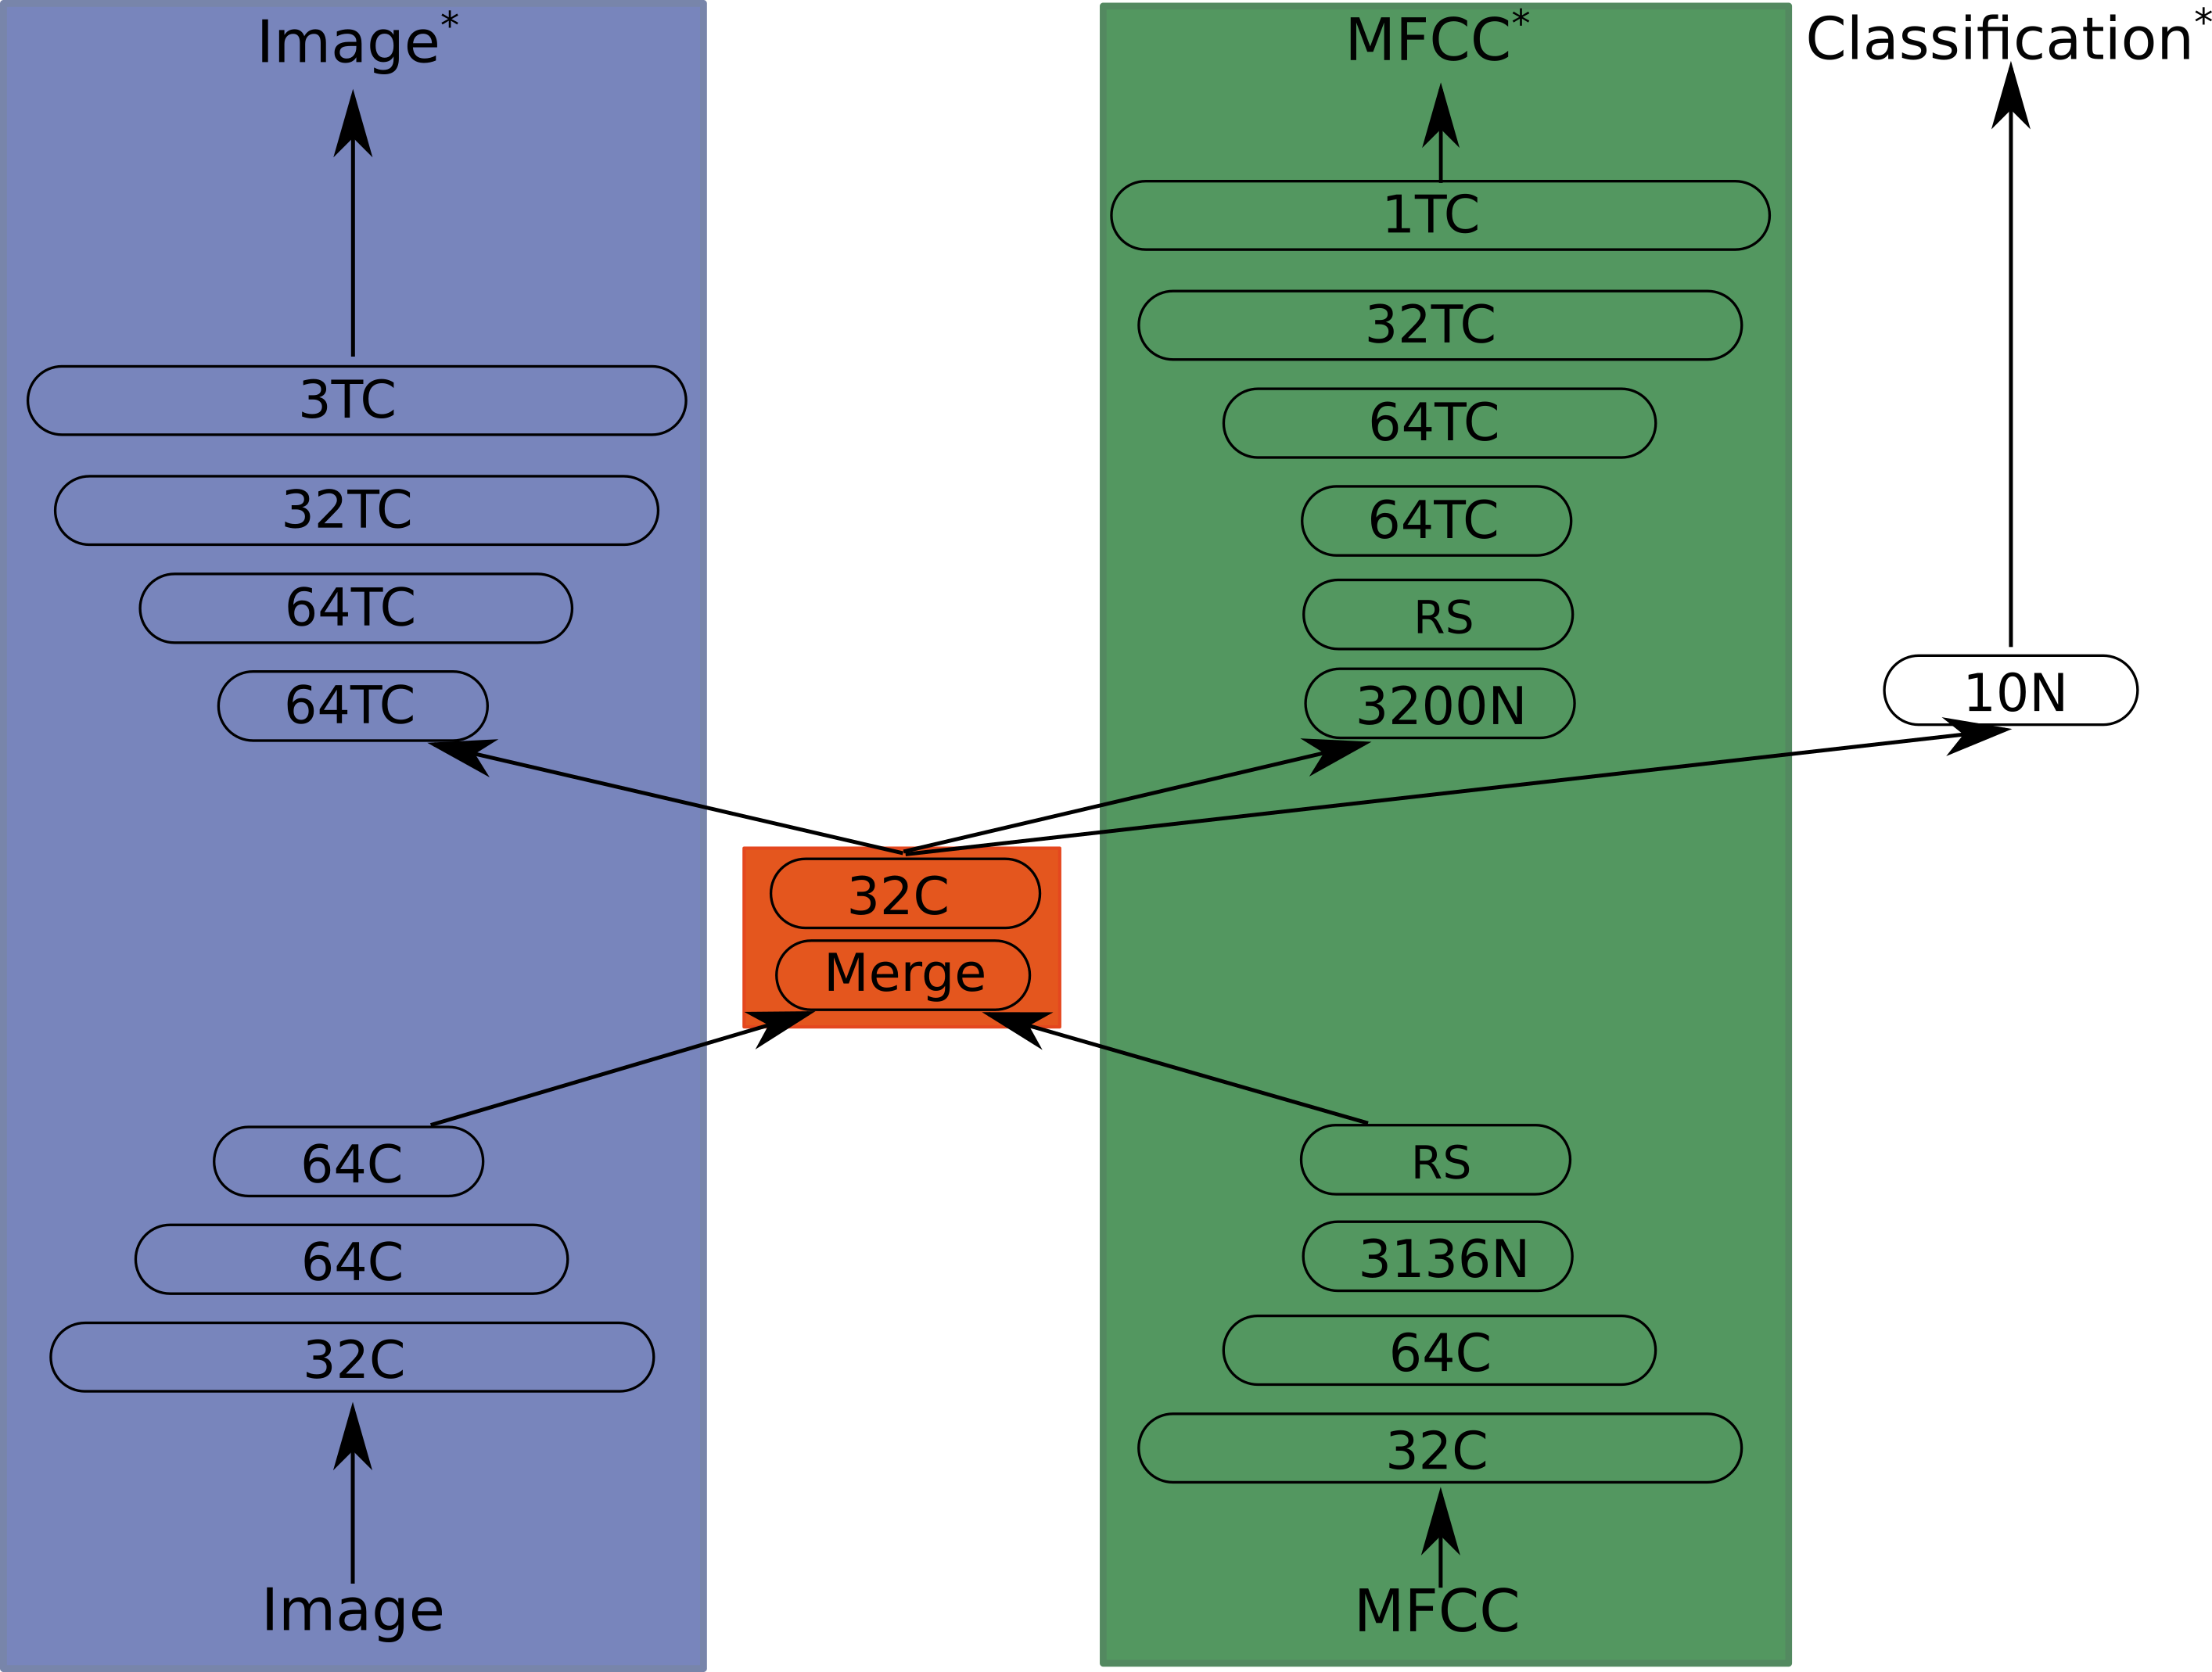
\includegraphics[width=0.75\textwidth]{Figs/mnistSpoken/grounderW2V.png}
\caption{\textcolor{red}{The \ac{MAE} architecture used to bidirectionally ground the MNIST and UCU datasets. Layers marked with C are convolution TC, Transposed Convolution, RS, Reshape and N, Dense.}}
\label{fig:netMnist}
\end{figure}

\textcolor{red}{\autoref{fig:netMnist} depicts the \ac{MAE} described in \autoref{tab:UCU_MNIST_MAE_description}. The blue box shows the portion of the \ac{MAE} which encodes and decodes images, whilst the green portion handles the MFCC data. The orange box is where the joint representation is formed. Inputs are labelled, Image and MFCC with their respective outputs being marked with an asterisk. The final output is the classification which is created by passing the joint representation to a single dense layer containing 10 neurons.}

\subsection{Results}

\subsubsection{Classification Results}
The complete set of results for this experiment are available in \autoref{tab:mnist_ucu_master_res} in \autoref{appendix:app4}. The most important results are shown in the following three tables: \autoref{tab:mnist_ucu_bi_res} for the Bimodal testing condition, \autoref{tab:mnist_ucu_im_res} for the Image Only condition and \autoref{tab:mnist_ucu_mfcc_res} for the \ac{MFCC} Only testing condition. 

All results reported here are the mean of a four-fold cross validation. Each training and testing condition was run four times and the average results are shown.


\begin{table}[h]
	\centering
		\begin{tabular}{|c|c|c|c|c|}
		\hline
		\textbf{Model} & \textbf{Training} & \textbf{Im MSE} & \textbf{MFCC MSE} &  \textbf{Acc} \\ \hline
				Image AE & Im & 	\textbf{0.0027}	&	       			& 	0.9883			\\ \hline		
				MFCC AE & MFCC & 		    		& 	\textbf{0.0113} &	0.9832			\\ \hline		
\multirow{2}{*}{Add MAE} & Bi & 	0.0030			&	0.0401			&	0.9967			\\ \cline{2-5}
						  & RR &	0.0033			&	0.0176			&	\textbf{0.9993}	\\ \hline	
		
\multirow{2}{*}{Concat MAE} & Bi & 0.0031			&	0.0423			&	0.9945			\\ \cline{2-5}		
							 & RR & 0.0030			&	0.0426			&	0.9986			\\ \hline
		\end{tabular}
		\caption{Mean Squared Errors for the Bimodal testing condition, comparing the Bimodal (Bi) and Randomly Removed (RR) training procedures.}
		\label{tab:mnist_ucu_bi_res}

\end{table}

In \autoref{tab:mnist_ucu_bi_res} it can be seen that both concatenate and addition merging produce models with better prediction accuracy than the baseline models, regardless of training procedure.

\begin{table}
	\centering
		\begin{tabular}{|c|c|c|c|}
		\hline
		\textbf{Model} & \textbf{Training} &  \textbf{MFCC MSE} &  \textbf{Acc} \\ \hline
		Image AE & Im 		&  		    			& \textbf{0.9883}	\\ \hline		
\multirow{2}{*}{Add MAE} & Bi & 	0.1641			& 0.4501 			\\ \cline{2-4}
						  & RR & \textbf{0.0455}	& 0.9834 			\\ \hline	
		
\multirow{2}{*}{Concat MAE} & Bi & 	0.2029		&	0.3496 			\\ \cline{2-4}		
							 & RR & 	0.0737		&	0.9834 			\\ \hline
		\end{tabular}
		\caption{Mean Squared Errors for the Image Only testing condition, comparing the Bimodal (Bi) and Randomly Removed (RR) training procedures.}
		\label{tab:mnist_ucu_im_res}

\end{table}

In comparison to the results in \autoref{tab:mnist_ucu_bi_res}, the results in \autoref{tab:mnist_ucu_im_res} show that the \acp{MAE} trained using the Bi training procedure do not generalise well when only a single input modality is available. Whereas the \acp{MAE} trained using the RR training procedure perform almost as well as the baseline model. 
\begin{table}[h]
	\centering
		\begin{tabular}{|c|c|c|c|}
		\hline
		\textbf{Model} & \textbf{Training} & \textbf{Im MSE} &  \textbf{Acc} \\ \hline
				
				MFCC AE & MFCC & 					& 	\textbf{0.9832}	\\ \hline		
\multirow{2}{*}{Add MAE} & Bi & 	0.1138			& 	0.9624 			\\ \cline{2-4}
						  & RR &	0.0556			&	0.9789			\\ \hline	
		
\multirow{2}{*}{Concat MAE} & Bi &	0.1138			&	0.9455			\\ \cline{2-4}		
							 & RR & \textbf{0.0554}	& 	0.9827 			\\ \hline
		\end{tabular}
		\caption{Mean Squared Errors for the MFCC Only testing condition, comparing the Bimodal (Bi) and Randomly Removed (RR) training procedures. }
		\label{tab:mnist_ucu_mfcc_res}

\end{table}

Similarly, the results in \autoref{tab:mnist_ucu_mfcc_res} show that the behaviour of the \ac{MAE} is very similar under the RR training procedure whether it is \acp{MFCC} or images provided as input. However, the classification accuracy does remain good, at 94.6\%, under the Bi training procedure when only \acp{MFCC} are present. 

\subsubsection{Reconstruction Results}

In \autoref{fig:mnistDigits} examples of reconstructed digits generated by both the \textit{Add} and \textit{Concat} \acp{MAE} are shown.

\begin{figure}[h]
\begin{center}
	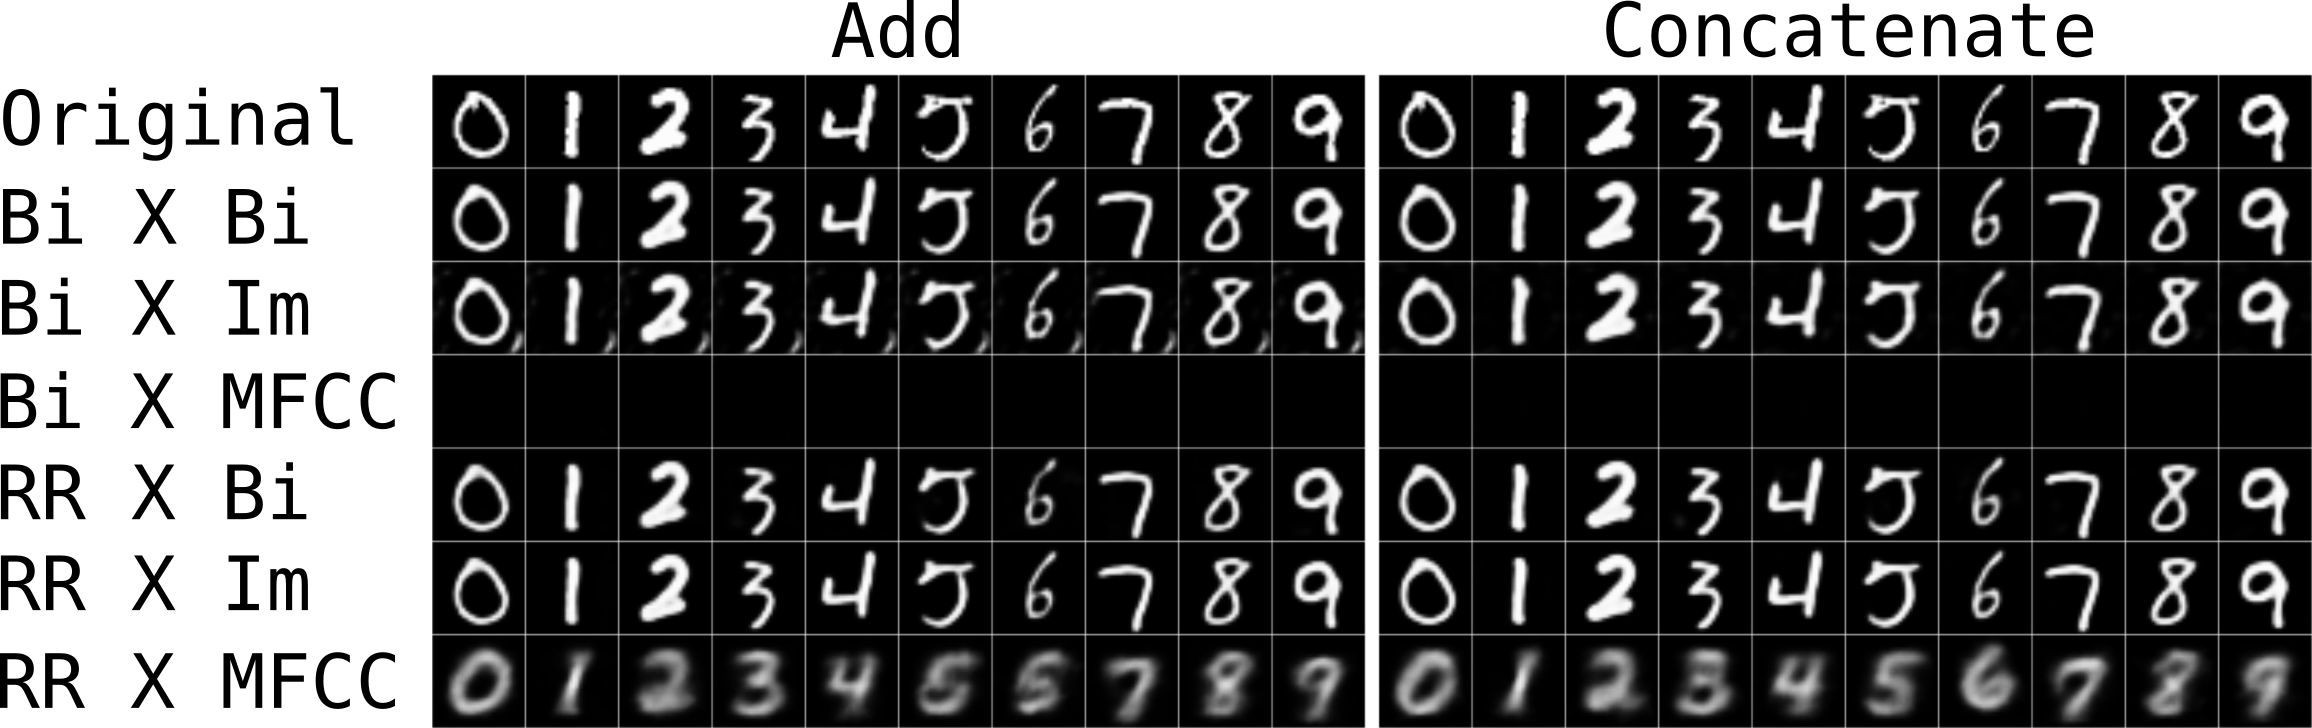
\includegraphics[width=\textwidth]{Figs/mnistSpoken/lbAll.png}
	\caption{A selection of randomly sampled digits generated in different training and testing conditions for both \textit{Add} and \textit{Concat} merging methods.}
	\label{fig:mnistDigits}
\end{center}
\end{figure}

\autoref{fig:5s} shows a comparison of two different examples of the digit ``5''. One is (subjectively) poorly written and the other is more prototypical and well formed. Under different testing conditions, the \acp{MAE} regenerate different ``fives''.

\begin{figure}[h]
\begin{center}
	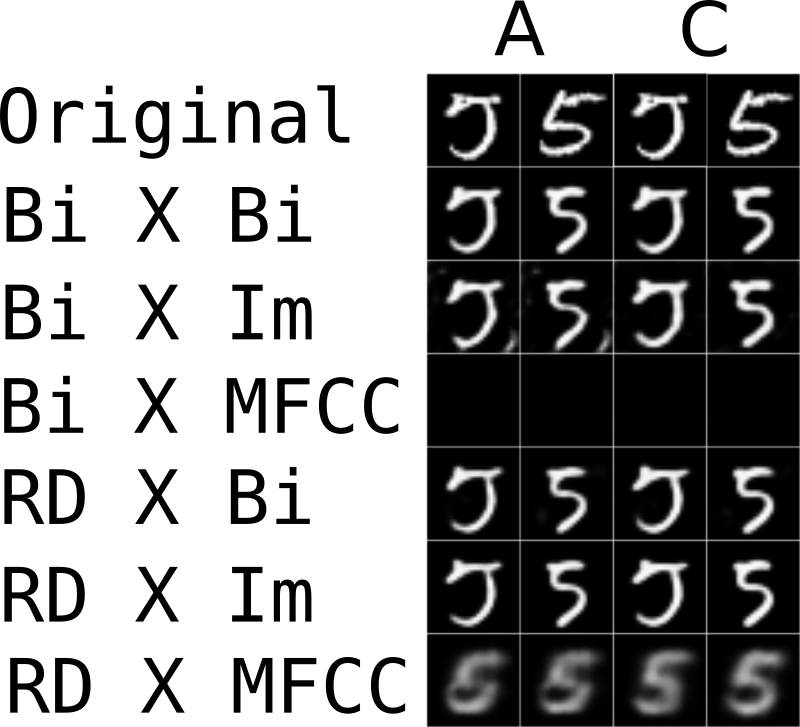
\includegraphics{Figs/mnistSpoken/5s.png}
	\caption{Two examples of the digit ``5'' being generated in different training and testing conditions for both \textit{Add} and \textit{Concat} merging methods.}
	\label{fig:5s}
\end{center}
\end{figure}



\subsection{Discussion}

\subsubsection{Discussion of Classification Results}
\autoref{tab:mnist_ucu_bi_res} shows that both the \textit{Add} and \textit{Concat} \acp{MAE} have better classification accuracy than the baseline, unimodal models. However, it is not clear that there is a difference between the two training procedures, Bi and RR.

The difference between the two training procedures becomes clear in \autoref{tab:mnist_ucu_im_res} where it can be seen that the \acp{MAE} trained using the Bi training procedure have lower classification rates when presented with only images as input. Models perform less than half as well as the baseline model, 0.4501 (\textit{Add}) and 0.3496 (\textit{Concat}) versus 0.9832 for the baseline image autoencoder. \textcolor{red}{This means that out of 100 thousand sample images, only 4501 were correctly classified by the \textit{Add} \ac{MAE} and 3496 were correctly classified by the \textit{Concat} \ac{MAE} compared to 9832 correctly classified by the baseline model.}

There is a trade off between unimodal accuracy and mulitmodal accuracy in the RR training procedure \acp{MAE}. Whilst both the \textit{Add} and \textit{Concat} \acp{MAE} outperform the baseline models in the Bimodal test condition, they have slightly worse performance when tested with either images or \acp{MFCC} only. For example, the best performance is given by the \textit{Add} \ac{MAE} under the RR training procedure when both images and \acp{MFCC} are present as inputs, with an accuracy of 0.9993 \textcolor{red}{(Only 7 samples incorrectly classified)}. However, if one of the modalities is removed, the accuracy drops to 0.9834 \textcolor{red}{(166 samples incorrectly classified)} and 0.9789 \textcolor{red}{(211 samples incorrectly classified)} for Image Only and \ac{MFCC} Only testing respectively. Comparing this to the baseline unimodal models, which have classification accuracies of 0.9883 \textcolor{red}{(117 samples incorrectly classified)} and 0.9832 \textcolor{red}{(168 samples incorrectly classified)} for image and \ac{MFCC} autoencoders respectively, it can be seen that there is a small decrease in performance for the MAEs tested with unimodal data compared to the unimodal baselines. 

There is a drop of 0.0049 and 0.0043 for Image Only and \ac{MFCC} Only testing using the \textit{Add} \ac{MAE}. \textcolor{red}{This leads to an additional 49 (Image Only) and 43 (MFCC Only) samples being incorrectly classified} However, this reduction in performance is counterbalanced by the improvement in performnace when both modalities are present, 0.9993 versus the 0.9883 and 0.9832 of the baseline models \textcolor{red}{i.e. an additional 110 images and 124 MFCC samples are correctly classified by the multimodal model compared to the unimodal baselines}. This improvement of 0.0110 to 0.0161 over the baseline image and \ac{MFCC} autoencoders is more than twice the decrease in performance when only one modality is available. 

Specifically, the improvement of Bimodal classification is 2.24 times larger than the decrease in performance when only images are available ($0.011 / 0.0049 = 2.24$). Comparing to the \ac{MFCC} baseline, the Bimodal performance improvement is 3.74 times larger than the decrease in performance when only \acp{MFCC} are available.

\subsubsection{Discussion of Reconstruction Results}
Observing \autoref{tab:mnist_ucu_bi_res}, \autoref{tab:mnist_ucu_im_res} and \autoref{tab:mnist_ucu_mfcc_res} it can be seen that different models have different reconstruction errors (Mean Squared Error). Whilst all \ac{MAE} models had higher reconstruction errors than the baseline models, this is to be expected. The \ac{MAE} models are trading off between representing each modality well, whilst the unimodal autoencoders that give the baseline numbers can use their full capacity to minimise the reconstruction error of their one modaility, as they do not have to reconstruct the second modality. 

That being said, the image reconstruction error is comparable across all \ac{MAE} models, approximately 0.0031, (see table \autoref{tab:mnist_ucu_bi_res} and is very close to the baseline of 0.0027 under the Bimodal testing condition (i.e. when the images to be reconstructed are available as input). Further to this, the image reconstruction error for the \ac{MFCC} Only testing condition is still small (0.0554), though an order of magnitude worse, for the \acp{MAE} trained using the RR procedure. \textcolor{red}{For context, the maximum \ac{MSE} would be one as the output is constrained to be between zero and one. So, if a generated sample was all black, that is all zeros and the desired output was all white, that is all ones, the \ac{MSE} would be $\frac{1}{i \times j}\sum_{i,j}({x_{i,j} - x*_{i,j}})^2 = 1$, where $i$ and $j$ are pixel coordinates and $x_{i,j}$ is one  and $x*_{i,j}$ is zero for all $i$ and $j$.}

\paragraph{Image reconstruction from MFCCs}
The increase in image reconstruction error when only \acp{MFCC} are provided as input is due to the construction of an internal symbolic language which represents the meaning of both the utterances (\acp{MFCC}) and images but not necessarily their fine details. For example, looking at \autoref{fig:5s} we see that there are different ways to write the number 5, however both of these images have the same meaning, ``five''. It is more important to preserve this meaning than the minutia of the original images. The same can also be said for reconstructing \acp{MFCC}, their meaning is more important than their exact enunciation.  

The \ac{MFCC} reconstruction error is best for the baseline model but is only 4.0265 times worse for the best performing model on this task (\textcolor{red}{0.0113 versus 0.0455}). Considering how small the baseline error is \textcolor{red}{(approximately 1.1\%)}, being four times worse, is still good performance, especially considering the difficulty of the task. 

\paragraph{MFCC reconstruction from Images}
The \ac{MFCC} reconstruction error is an order of magnitude worse than the image reconstruction error. In part this is due to the nature of the data, as seen by the difference in baseline reconstruction errors. It appears to be more difficult to reconstruct \acp{MFCC} than images, even when \acp{MFCC} are given as input.

Another contributing factor to the worse \ac{MFCC} reconstruction error for the \acp{MAE}, is the inbalance between sample numbers for MNIST and UCU. Whilst both datasets are balanced within themselves (there are an equal number of training samples for each class) there is a big difference between the sizes of MNIST and UCU. 

The difference in sizes between the datasets means that reconstructing \acp{MFCC} from image inputs will map a large number of inputs to a smaller number of outputs and vice-versa for generating images from \ac{MFCC} inputs. Therefore images in the test set which look similar to images in the training set, will be mapped to \acp{MFCC} similar to those which the training images map too. As there are a smaller number of \ac{MFCC} examples to map to, our output is less likely to be normally distributed. Whilst idealy we would like to map similar looking digits to similar sounding utterances, there is no gaurantee that this is true, either in our dataset or in general. People with similar handwritting don't necessarily have similar voices. This is simulated by the random assignment of images to \acp{MFCC} but this results in discontinuities in the latent space of the network, particularly with respect to generating \acp{MFCC}, of which we have fewer examples to capture the true distribution of the data.

Conversely, as there are more examples of images of digits, the distribution of the latent space with respect to the images can get closer to modelling the real distribution of the images. Therefore, given a test \ac{MFCC}, regardless of whether it is similar to a training \ac{MFCC} example, its target image, is more likely to be similar to images in the training data. 

\paragraph{Effects of randomly removing inputs}
\autoref{fig:mnistDigits} shows that randomly removing the training data has a significant effect, beyond just the improvements to classification accuracy seen in \autoref{tab:mnist_ucu_bi_res}, \autoref{tab:mnist_ucu_im_res} and \autoref{tab:mnist_ucu_mfcc_res}. Both the \textit{Add} and \textit{Concat} \acp{MAE} fail to learn to generate images from \ac{MFCC} data using the Bi training procedure.

Comparing the images generated by the \textit{Add} and \textit{Concat} \acp{MAE} (\autoref{fig:mnistDigits}) for the \ac{MFCC} test condition when the training data has been Randomly Removed, it can be seen that the \textit{Concat} \ac{MAE} outperforms the \textit{Add} \ac{MAE}. This is particularly clear when you look at the ``five'' and ``six'' generated by the \textit{Add} \ac{MAE} for RR X \ac{MFCC} \textcolor{red}{(highlighted in red)}, where the \ac{MAE} has failed to correctly generate a ``six'' and has instead generated a ``five'', which is similar to the prototypical five generated when \acp{MFCC} for a five are presented.
Unlike the \textit{Add} \ac{MAE}, the \textit{Concat} \ac{MAE}, correctly generates all digits, including ``six''.

\paragraph{Multiple generations of the same digit}
In \autoref{fig:5s} we see that different examples of the same digit produce different generation results. Most interestingly however, are the generated ``fives'' shown in the RR X MFCC row. A more prototypical ``five'' is generated from \acp{MFCC} than if an image of a non-prototypical five is given. This shows that the meaning of the \acp{MFCC} have been grounded in the image modality and that an internal symbolic language has been learnt, i.e. the latent embedding of \acp{MFCC} are a symbolic representation which has meaning in both \ac{MFCC} and image space, hence the ability to generate meaningful images and \acp{MFCC} from these embeddings.

\textcolor{red}{In \cite{lupyan2007reuniting} it was demonstrated that adding a labelling to a visual symbol improved the speed at which it was identified by adults. From \autoref{fig:5s} it can be seen that the addition of the MFCCs as a labelling for the images has a similar effect when trying to classify digits with the \ac{MAE}. The MFCCs have the effect of altering the representation of the digit within the network closer to the representation of the mean of the class. I.e. testing with MFCCs alone leads to the generation of prototypical digits. The representation of these digits is more eaily recognisable than non-prototypical representation (e.g. those representing images of outlier digits like the first 5 in \autoref{fig:5s}). The \ac{MAE} combines the prototypical representation generated from the MFCCs with the non-prototypical representation of the image creating a joint representation which is more easily recognisable as belonging to a specific class.}

\section{Summary}
In this chapter I set out to demonstrate the advantages of multimodality as applied to classification and regeneration of missing data.

Whilst multimodal systems can provide better classification accuracy, this comes at the cost of a higher computational burden and, lower classification accuracy when only one modality is available, as demonstrated by the results presented in this chapter. \textcolor{red}{This demonstrates that whilst MRL can enhance classification accuracy, proving hypothesis 2, it does come with trade-offs.}

The ability to reconstruct missing data from a secondary modality demonstrates how an internal symbolic language can be learnt in an unsupervised fashion by processing aligned percepts in multiple modalities \textcolor{red}{proving hypothesis 1 to be true}.

In future it would be worth while to observe how the reconstructed data can be exploited to improve classification accuracy, for example by first generating a missing data points from modality A and then performing a classification on the embedding of data from modality B and the generated modality A.

This experiment lays the ground work for the next chapter where I will look at how a more complex internal symbolic language can be developed and exploited.

Further discussion of the results from this chapter have been published in \cite{sheppardtowards}. 
%I will also discuss how this can be applied to creating robots capable of life long learning. 
